\subsubsection{Community}
La sezione Community corrisponde alla ex "Esplora Appunti" della versione
precedente, rinominata per comunicare più chiaramente la sua funzione di spazio condiviso tra utenti. Il layout adottato è il medesimo della sezione "Appunti", scelta che ha permesso di mantenere coerenza visiva tra le due sezioni e di applicare in parallelo alcune delle stesse modifiche: la rimozione della vista a griglia in favore della sola vista a lista, la barra di ricerca per titolo affiancata dai filtri per
metadati e la ridefinizione delle colonne di visualizzazione dei file. Le modifiche specifiche alla sezione Community riguardano invece la gestione della distinzione tra contenuti propri e altrui e la scelta di non introdurre strumenti di organizzazione personale come le cartelle, per mantenere una separazione netta rispetto allo spazio personale già offerto da "Appunti".

\paragraph{Modifiche progettuali}
La visualizzazione a griglia è stata rimossa in favore della sola vista a lista, in quanto risultava inadatta alla consultazione di grandi quantità di file: con decine o centinaia di documenti, la griglia mostra meno informazioni per elemento, presenta inconsistenze visive tra le due modalità e causa problemi di interazione. La vista a lista permette invece di esporre più metadati per ciascun file in modo uniforme, facilitando la scansione e il confronto rapido tra i risultati. \\

Problemi di usabilità risolti:
\begin{itemize}
  \item P36 (Cliccando sull'icona del documento non succede nulla, bisogna cliccare il bordo della card): Con la rimozione della vista a griglia il problema non è più riproducibile.
  \item P37 (In vista griglia mancano data di caricamento e università): La vista a lista espone uniformemente tutti i metadati per ciascun file.
  \item P38 (Il pulsante "Scarica" cambia aspetto tra vista lista e vista griglia): Con la rimozione della vista a griglia il problema non è più riproducibile.
  \item P39 (Il nome dell'autore cambia aspetto tra vista lista e vista griglia): Con la rimozione della vista a griglia il problema non è più riproducibile.
\end{itemize}

\begin{figure}[H]
  \centering
  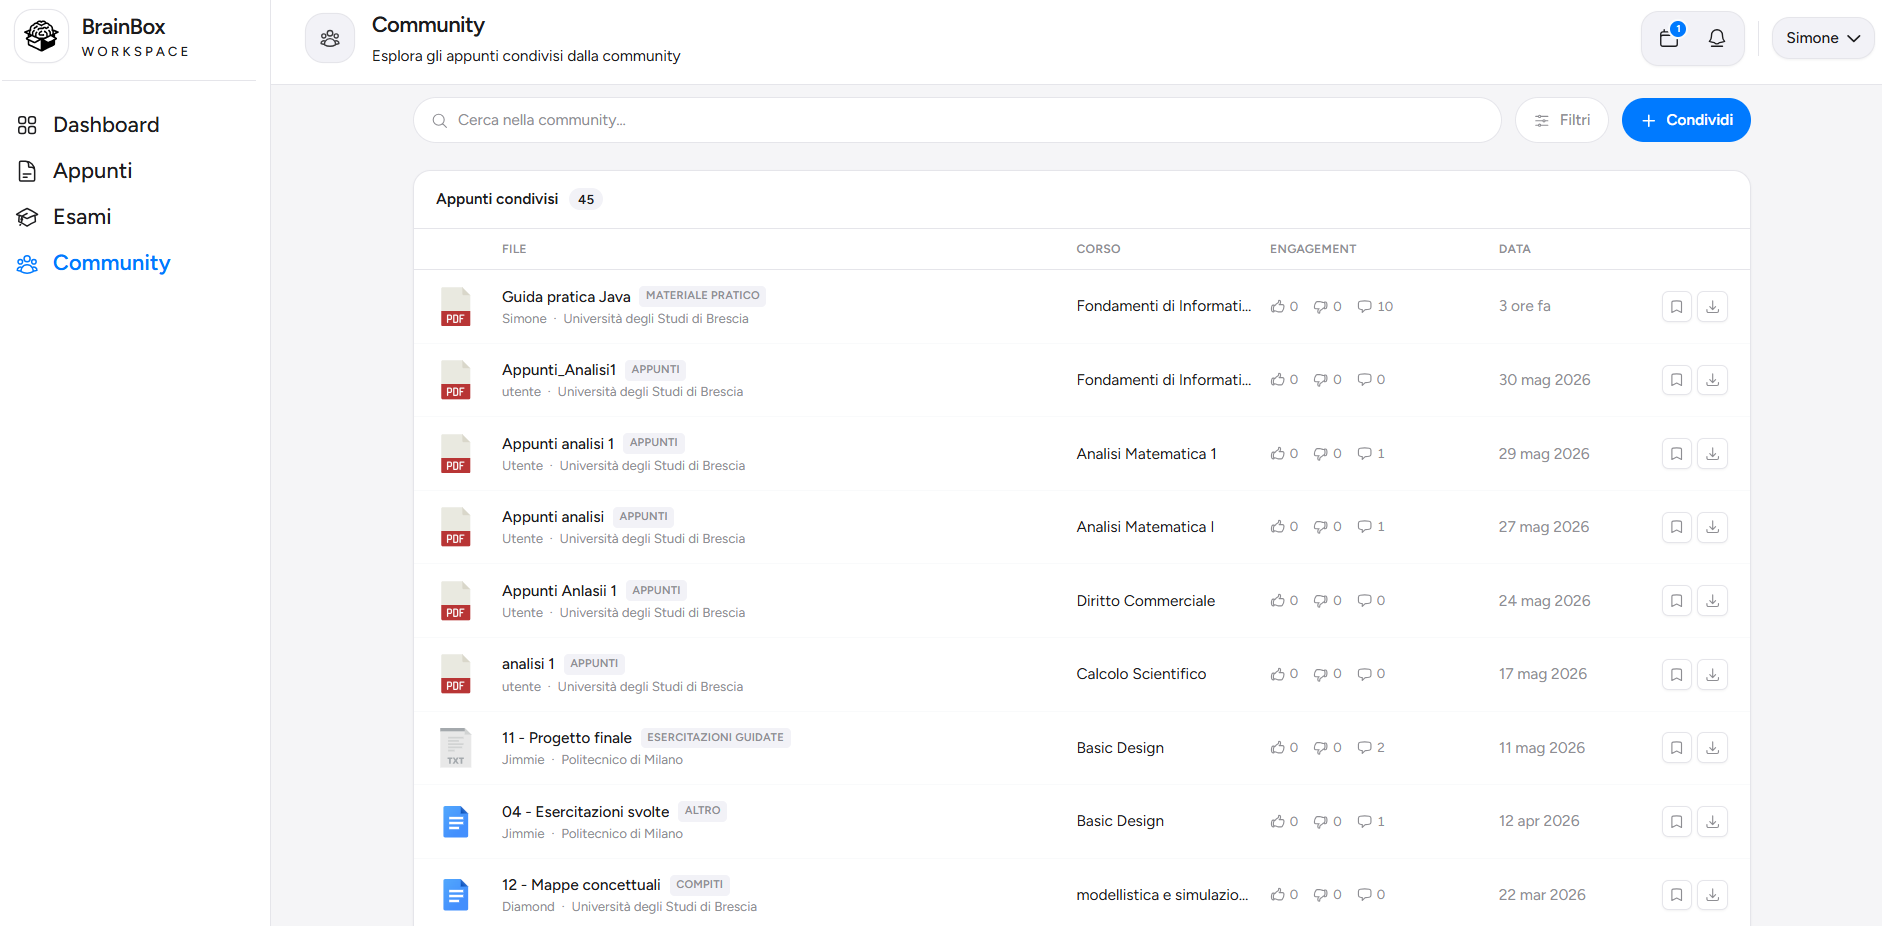
\includegraphics[width=0.8\textwidth]{figures/fig-riprogettazione-fisica/community/community_1.png}
  \caption{Vista a lista sezione Community}
  \label{fig:community_1}
\end{figure}

La barra di ricerca è stata mantenuta per la ricerca per titolo e sono stati aggiunti o corretti i filtri dedicati per i principali metadati, "Università", "Corso", "Categoria" e "Anno Accademico", per permettere all'utente di restringere i risultati lungo dimensioni multiple senza dover digitare query complesse. In questo modo l'utente può combinare liberamente ricerca testuale e filtri per individuare rapidamente i contenuti di interesse. \\

Problemi di usabilità risolti:
\begin{itemize}
  \item P52 (La ricerca è limitata al solo titolo del documento): Sono stati aggiunti o corretti i filtri per i principali metadati, ampliando le possibilità di ricerca.
  \item P57 (Nessun controllo sull'ordinamento e sul filtraggio delle liste): I filtri permettono all'utente di restringere i risultati secondo le dimensioni più rilevanti.
\end{itemize}

\begin{figure}[H]
  \centering
  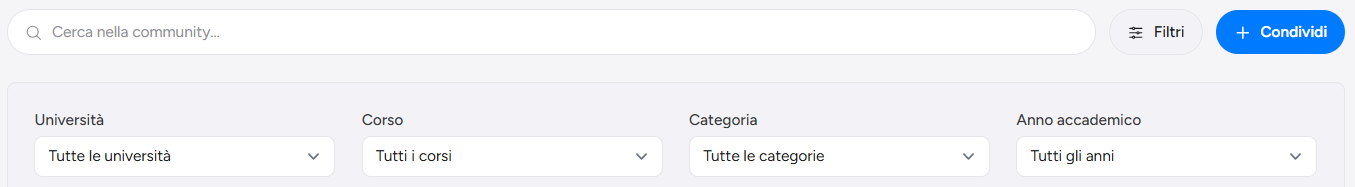
\includegraphics[width=0.8\textwidth]{figures/fig-riprogettazione-fisica/community/community_2.png}
  \caption{Filtri di ricerca della Community}
  \label{fig:community_2}
\end{figure}

La distinzione tra i propri contenuti condivisi e quelli degli altri utenti è stata risolta a livello strutturale tramite i tab della sezione Community. La vista predefinita mostra tutti i documenti condivisi sulla piattaforma, mentre selezionando il tab "Appunti condivisi" viene applicato un prefiltro che mostra esclusivamente i documenti
pubblicati dall'utente stesso. \\

Problemi di usabilità risolti:
\begin{itemize}
  \item P69 (Nessuna distinzione visiva tra proprie risorse e risorse altrui): La distinzione è gestita tramite il tab "Appunti condivisi" che applica un prefiltro sui soli documenti pubblicati dall'utente, senza necessità di distinguerli visivamente all'interno della lista generale.
\end{itemize}

\begin{figure}[H]
  \centering
  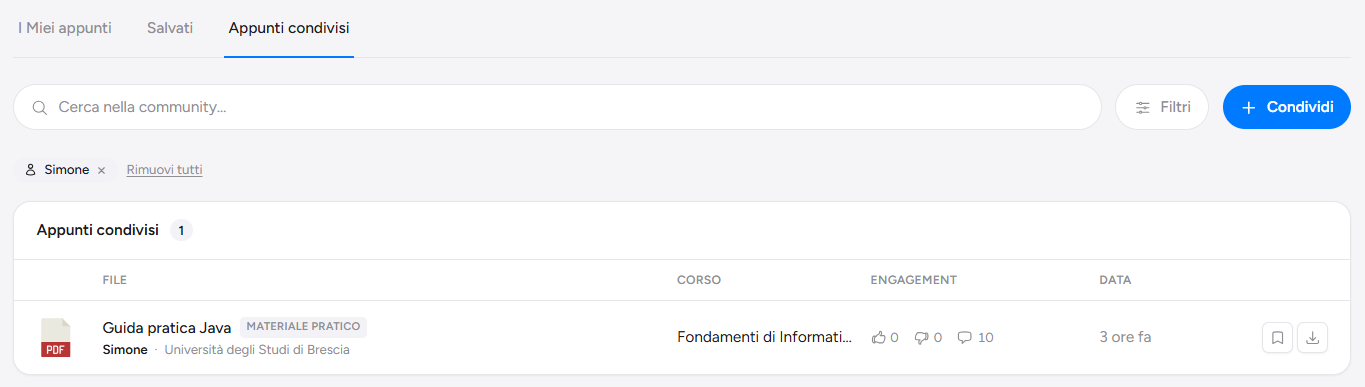
\includegraphics[width=0.8\textwidth]{figures/fig-riprogettazione-fisica/community/community_3.png}
  \caption{Tab "Appunti Condivisi"}
  \label{fig:community_3}
\end{figure}

È stato introdotto un feedback visivo per distinguere i file già visualizzati
da quelli non ancora consultati. \\

Problemi di usabilità risolti:
\begin{itemize}
  \item P61 (Nessun feedback visivo sui file già visualizzati): È stata introdotta una distinzione visiva tra file già aperti e file non ancora consultati: i primi vengono visualizzati con opacità ridotta, in modo che i contenuti nuovi risaltino immediatamente all'interno della lista. La modifica è stata applicata in modo coerente anche nella sezione "Appunti".
\end{itemize}
